\documentclass[UTF8]{article}
% Template based on https://www.overleaf.com/latex/templates/assignment-template/fwycphfzpshm

\usepackage[authoryear]{natbib}
\usepackage{url}
\usepackage{amsmath}
\usepackage{amsfonts}
\usepackage[margin=1in]{geometry}
\usepackage{multirow}
\usepackage{graphicx}
\usepackage{pdfpages}

\title{AttentiveCLS Pooler}
\author{
  Team 1:  % team no
  Seungil Lee, Jongchan Park, Eugene Seo, and Dohyung Kim % your names
}
\date{\today}

\begin{document}
\maketitle

\section{Introduction}

BERT~\cite{devlin-etal-2019-bert} has become a standard architecture for NLP research ever since it was published. BERT computes the representation for every token, but it uses the output representation of the special token \texttt{[CLS]}, for sentence-level tasks (e.g., sentiment analysis). However, various strategy can be applied to get sentence-level representation, so we are going to design new method and try some of them in this homework.

We have designed new pooler named \texttt{AttentiveCLS} pooler and evaluated its performance on CoLa, MNLI and MRPC tasks, which are the representatives of sentence-level tasks. The results were compared with \texttt{MeanMaxTokens} pooler, which is suggested in the homework description, also with the original \texttt{BERTPooler} in \texttt{huggingface} library (\url{https://huggingface.co/}).

\section{AttentiveCLS Pooler}
Though original BERT pooler simply adopts last output of \texttt{[CLS]} token, we tried to exploit information from other tokens as well. Nowadays, attention mechanism is widely used to get the importance of the given sequence, so we added a attention pooling layer on the top of the tokens other than \texttt{[CLS]} token. Then, the output of this attention layer is concatenated with the last output of \texttt{[CLS]} token.

We also apply linear transformation with $W \in \mathbb{R}^{H \times 2H}$ and $\tanh$ activation just like as the \texttt{BERTPooler} in \texttt{huggingface} implementation.

The \texttt{BERTPooler} in \texttt{huggingface} implementation applies linear transformation with $W \in \mathbb{R}^{H \times H}$ and $\tanh$ activation (See \texttt{BertPooler} class). Similarly, we apply linear transformation with $W_{\text{MMT}} \in \mathbb{R}^{H \times 2H}$ and $\tanh$ activation.

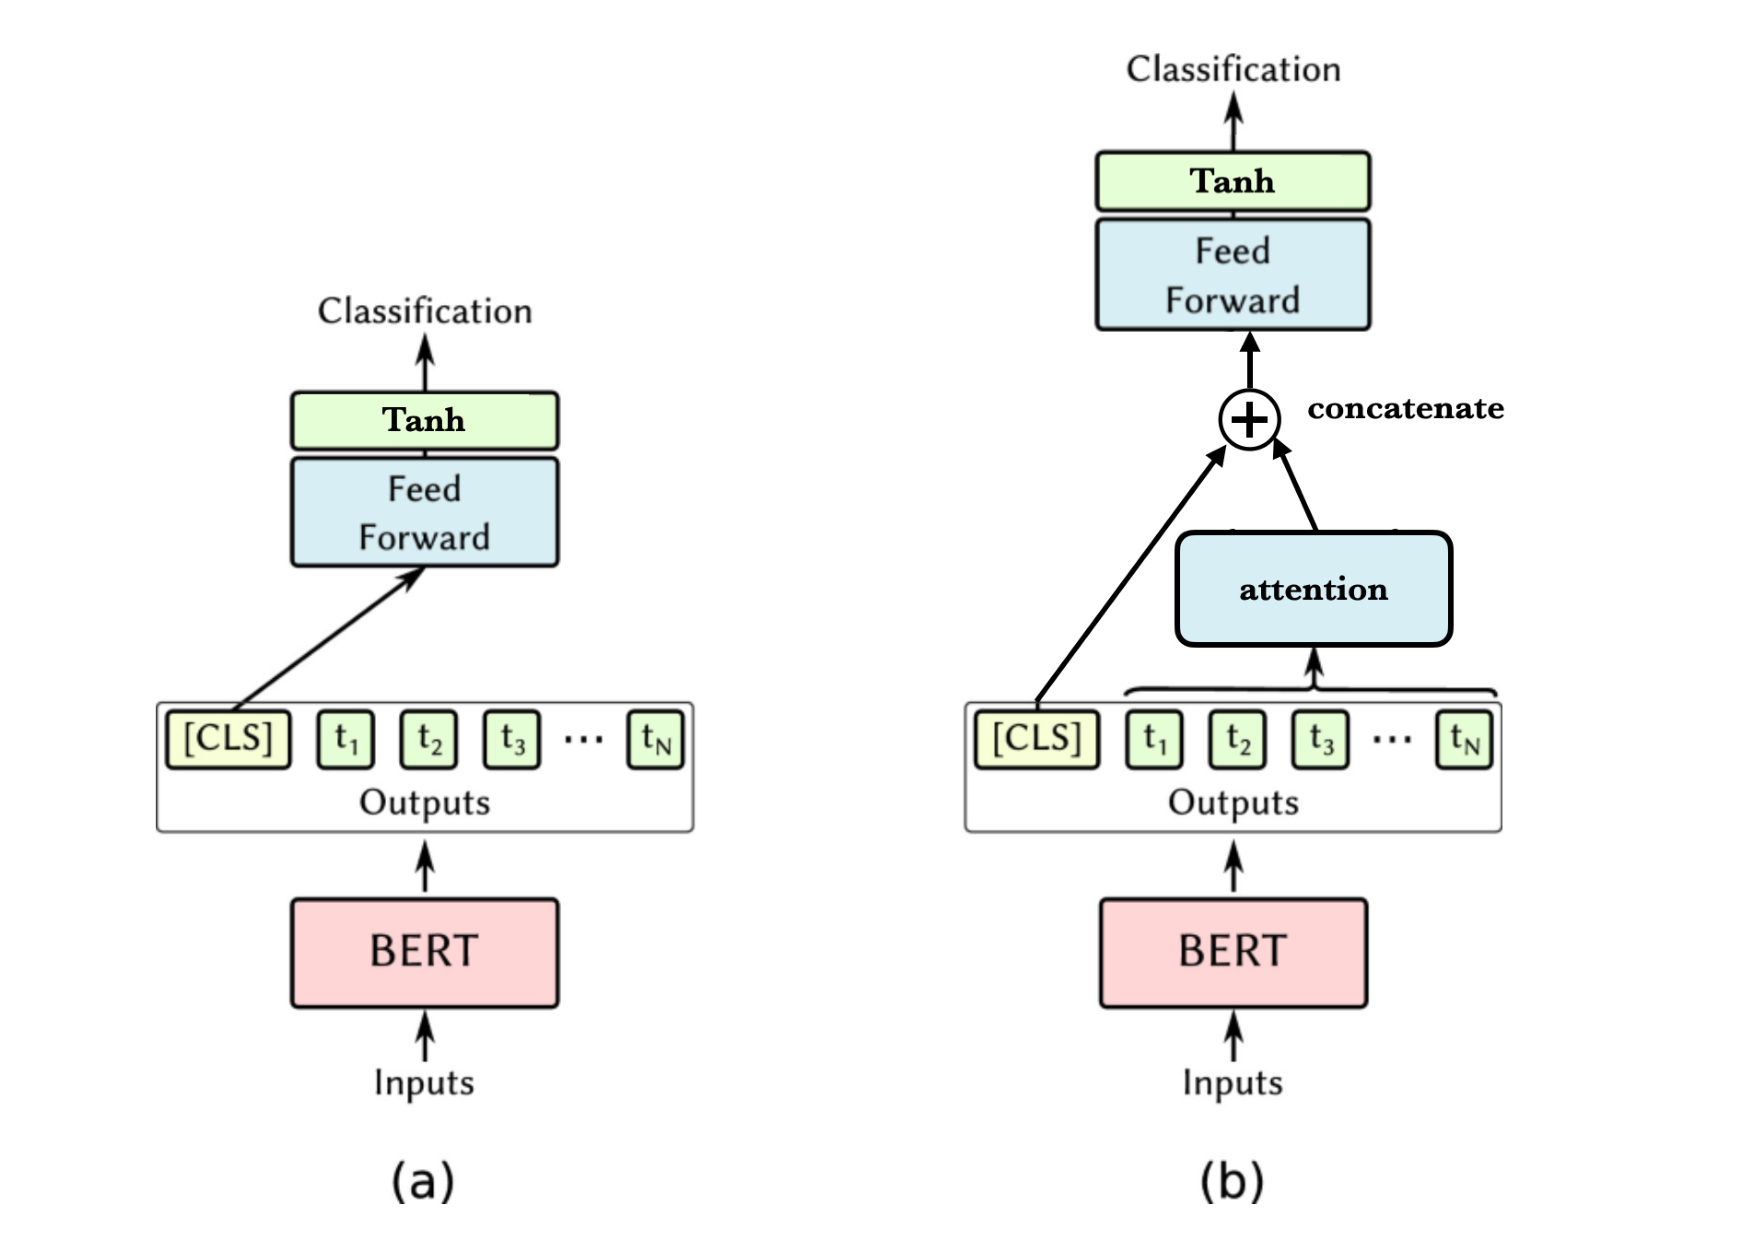
\includepdf[pages=-]{figure1.pdf}


The tasks in this homework are as follows:
\begin{enumerate}
  \item Implement the \texttt{MeanMaxTokens} pooler (See \texttt{MeanMaxTokensBertPooler} class in \texttt{bert\_poolers.py}).
  \item Implement your own BERT pooler (See \texttt{MyBertPooler} class) and describe its architecture and rationale in your report. It does not have to be completely novel.
  \item Choose one dataset in GLUE~\cite{wang2018glue}, and compare the test performance of three poolers (See \texttt{run\_glue.py}).
  \item Discuss the result. Negative results are fine, the point is how you interpret and explain it.
\end{enumerate}

\section{Experiment}


% \begin{table}[]
% \begin{tabular}{|l|ll|lll|ll|ll|}
% \hline
% \multirow{2}{*}{} & \multicolumn{2}{c|}{CoLA}                                                        & \multicolumn{3}{c|}{MRPC}                                                                               & \multicolumn{2}{c|}{RTE}                                         & \multicolumn{2}{c|}{SST-2}                                       \\ \cline{2-10} 
%                   & \multicolumn{1}{c|}{Loss}            & \multicolumn{1}{c|}{matthews_correlation} & \multicolumn{1}{c|}{Accuracy}        & \multicolumn{1}{c|}{F1}              & \multicolumn{1}{c|}{Loss} & \multicolumn{1}{c|}{Accuracy}        & \multicolumn{1}{c|}{Loss} & \multicolumn{1}{c|}{Accuracy}        & \multicolumn{1}{c|}{Loss} \\ \hline
% AttentiveCLS      & \multicolumn{1}{l|}{0.4588}          & \textbf{0.6004}                           & \multicolumn{1}{l|}{\textbf{0.8554}} & \multicolumn{1}{l|}{\textbf{0.9012}} & \textbf{0.3952}           & \multicolumn{1}{l|}{0.6173}          & 0.7498                    & \multicolumn{1}{l|}{0.9289}          & 0.3272                    \\ \hline
% MeanMax           & \multicolumn{1}{l|}{\textbf{0.4208}} & 0.5735                                    & \multicolumn{1}{l|}{0.8162}          & \multicolumn{1}{l|}{0.8777}          & 0.4424                    & \multicolumn{1}{l|}{0.5379}          & \textbf{0.6920}           & \multicolumn{1}{l|}{\textbf{0.9312}} & 0.2711                    \\ \hline
% BERTPooler        & \multicolumn{1}{l|}{0.4388}          & 0.5934                                    & \multicolumn{1}{l|}{0.8456}          & \multicolumn{1}{l|}{0.8934}          & 0.4000                    & \multicolumn{1}{l|}{\textbf{0.6462}} & 0.7058                    & \multicolumn{1}{l|}{0.9300}          & \textbf{0.2387}           \\ \hline
% \end{tabular}
% \end{table}

The files you should submit are
\begin{enumerate}
  \item Your team's \texttt{bert\_poolers\_\{team\_no\}.py} (e.g, \texttt{bert\_poolers\_0.py}).
  \item Your team's two-page \texttt{report\_\{team\_no\}.pdf} (e.g., \texttt{report\_0.pdf}). Use this \LaTeX\ file as a template, and do not change style attributes in this file. References are not included in the page-limit.
\end{enumerate}


\section{Experiment}

Comprehensive evaluation based on clarity, validity, and interestingness. You will get zero points if you violate academic integrity (e.g., plagiarism and data manipulation).

\section{Result}


\bibliographystyle{plain}
\bibliography{report.bib}


\end{document}
